\documentclass[11pt]{article}

\usepackage[margin=1.1in]{geometry}

%An theloume na allaksoume to still ton paragrafon kai na tis kanoume opos sto word afairoume ta comments apo tis 2 parakato grammes
%\parindent 0mm
%\parskip=\baselineskip

\usepackage{hyperref}
\usepackage{bookmark}
\makeatletter
%An theloume na exoume arithmous sta sections, vazoume se comment tis 2 parakato grammes
\renewcommand\@seccntformat[1]{}
\makeatother

%Aparaitita paketa gia ellinika
\usepackage{xltxtra} 
\usepackage{xgreek} 
%I poly kali grammatoseira GFS Didot pou kanoun ta ellinika na miazoun stin grammatoseira tou LaTeX
\setmainfont[Mapping=tex-text]{GFS Didot} 
 
\title{\textbf{Τίτλος Εργασίας}}
\author{Όνομα Συγγραφέα \\ Όνομα Ινστιτούτου / Εταιρείας}
\date{}
\begin{document}
\maketitle

\section{Εισαγωγή}
%Dummy text
Ο Όμηρος είναι ο υποτιθέμενος συγγραφέας της Οδύσσειας (όπως και της Ιλιάδας), ο οποίος πιστεύεται οτι έζησε κατά τον 8ο ή 7ο αιώνα π.Χ. Η ύπαρξή του αμφισβητείται από κάποιους λόγιους που βλέπουν ασυμφωνίες στα δύο επικά ποιήματα, αλλά υποστηρίζεται από άλλους που βλέπουν τη συνολική συνέπεια και δηλώνουν οτι τα ποιήματα αυτά θα μπορούσαν να είναι μόνον το έργο μιας και μοναδικής ιδιοφυΐας. Αυτό που σίγουρα γνωρίζουμε είναι οτι τόσο η Ιλιάδα όσο και η Οδύσσεια υπέστησαν μια διεργασία τυποποίησης, ιδίως την εποχή του Αθηναίου τυράννου Ιππάρχου (6ος αι. π.Χ.), ο οποίος αναμόρφωσε την απαγγελία της Ομηρικής ποίησης. Σχεδόν τίποτε δεν είναι γνωστό για τον Όμηρο. Η Χίος, και αρχαίες ελληνικές πόλεις της δυτικής ακτής της Μικράς Ασίας έχουν υποστηρίξει οτι υπήρξαν γενέτειρές του. Όταν ο Ρωμαίος αυτοκράτορας Αδριανός ρώτησε το Μαντείο των Δελφών ποιος ήταν στ’ αλήθεια ο Όμηρος, η Πυθία απάντησε οτι ήταν από την Ιθάκη, γιος του Τηλέμαχου (του γιου του Οδυσσέα) και της Επικάστης. Αν ο Όμηρος υπήρξε, θα ήταν ίσως ένας τυφλός βάρδος. Αυτό συνάγεται από ένα επεισόδιο στη Ραψωδία Θ (8) που μπορεί να κάνει αυτο-αναφορά, όπου ο τυφλός βάρδος Δημόδοκος τραγουδά για το βασιλιά και το κοινό των Φαιάκων.

Η Οδύσσεια αποτελείται από 24 ραψωδίες (“κεφάλαια”). Λόγω του αριθμού-τους, σε κάθε μία δίνεται το όνομα ενός από τα 24 γράμματα του ελληνικού αλφαβήτου. Αρχικά δεν υπήρχε τέτοιος διαχωρισμός σε ραψωδίες (η πρακτική αυτή εισήχθη κατά τον 3ο αι. π.Χ.), και το ποίημα δεν ήταν καν γραπτό, μόνον απαγγελόταν, και περνούσε από γενεά σε γενεά μέσω της μνήμης. Εντούτοις, το ελληνικό αλφάβητο εισήχθη κατά τον 8ο αι. π.Χ., λίγο πριν τη γέννηση του Ομήρου (ή της Οδύσσειας), άρα είναι δυνατό να καταγράφηκε το ποίημα κάποια εποχή σύντομα μετά τη δημιουργία-του.

Το ποίημα περιγράφει το δεκάχρονο ταξίδι του βασιλιά Οδυσσέα, από τα πεδία μαχών της Τροίας στο βασίλειό του στην Ιθάκη. Ξεκινά στο μέσον του ταξιδιού του Οδυσσέα, όταν ο γιος-του Τηλέμαχος ταξιδεύει σε κοντινά βασίλεια ρωτώντας να μάθει για τον πατέρα-του, ενώ ο Οδυσσέας βρίσκεται στο νησί των Φαιάκων και διηγείται τα παθήματά του στο προηγούμενο μέρος του ταξιδιού. Όμως πίσω στην Ιθάκη, μνηστήρες πλησιάζουν τη σύζυγό του, βασίλισσα Πηνελόπη, κατασπαταλώντας την περιουσία-του καθώς μένουν στο παλάτι, και προσπαθώντας να πείσουν την Πηνελόπη να διαλέξει και να παντρευτεί έναν απ’ αυτούς. Εντωμεταξύ, με τη βοήθεια των Φαιάκων και της θεάς Αθηνάς, ο Οδυσσέας ετοιμάζεται να επιστρέψει στα πατρώα εδάφη-του.

\section{Κυρίως θέμα}

\subsection{Γνωστά Ζητήματα σχετικά με τον Κλασικό Αναγνώστη}

Γιατί στο αρχαίο κείμενο δεν αρχίζει η κάθε πρόταση με κεφαλαίο γράμμα μετά από τελεία;

Γιατί η πρακτική του να γράφουμε κεφαλαίο το πρώτο γράμμα μετά από τελεία είναι σχετικά πρόσφατη. Αν δείτε τα αρχαία κείμενα έτσι όπως τα έγραφαν οι αντιγραφείς (χειρόγραφα), θα διαπιστώσετε οτι δεν χρησιμοποιούσαν κεφαλαίο γράμμα μετά από τελεία.

Γιατί το κείμενο παρουσιάζεται μ’ αυτόν τον περίεργο τρόπο, με τα γράμματα να εμφανίζονται να “σμπρώχνουν” το ένα το άλλο μέχρις ότου μπει το καθένα στη θέση του;

\begin{figure}[h]
   \centering
       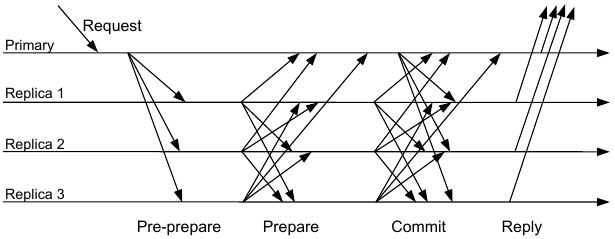
\includegraphics[width=0.8\textwidth]{protocol}
   \caption{Μία εικόνα.}
\end{figure}

Αυτό συμβαίνει μόνο στη μικροεφαρμογή Java αυτής της σελίδας (και όχι στο αυτόνομο πρόγραμμα), και γίνεται επειδή κάθε γράμμα είναι ένα εικονίδιο (GIF). Οι περιηγητές του διαδικτύου (όπως επίσης και η Java που είναι υπεύθυνη για την εμφάνιση αυτών των εικονιδίων στην οθόνη-σας) δείχνουν τις εικόνες με τυχαία σειρά, όταν υπάρχουν περισσότερες από μία στην ίδια σελίδα. Έτσι, οι εικόνες των γραμμάτων εμφανίζονται κι αυτές τυχαία, δηλαδή με τη σειρά που φορτώνονται από το διαδίκτυο, μέχρις ότου μπουν όλες στη θέση-τους. Από τη στιγμή πάντως που μια εικόνα έχει φορτωθεί δεν χρειάζεται να ξαναφορτωθεί όποτε εμφανίζεται, εκτός εάν βγείτε από την παρούσα σελίδα. Γιαυτό το λόγο αυτή η απρόσμενη συμπεριφορά μειώνεται μέχρι που παύει να υπάρχει καθώς προχωράτε στο κείμενο. Εντούτοις, το πρόβλημα αυτό δεν υπάρχει στο αυτόνομο πρόγραμμα, γιατί εκείνο δουλεύει τοπικά στον υπολογιστή-σας.

Μερικές φορές η χρήση των γραμμών ολίσθησης (scrollbars) του περιηγητή (όχι των έγχρωμων εσωτερικών του Κλασικού Αναγνώστη) χαλάει την εμφάνιση κάποιας γραμμής ή γραμμών του κειμένου.

Αυτό το πρόβλημα δημιουργείται από τον περιηγητή, και εμφανίζεται περιστασιακά όταν κάνουμε ολίσθηση (scroll) πάνω ή κάτω στην ιστοσελίδα, την ίδια ώρα που μια μικροεφαρμογή Java προσπαθεί να εμφανίσει τα περιεχόμενα που της έχουν ανατεθεί. Για να επανεμφανίσετε το κείμενο στη σωστή-του μορφή, κάντε κλικ στην επιλογή Κείμενο, και επιλέξτε το ίδιο κεφάλαιο με αυτό που διαβάζετε τώρα. Και πάλι, το πρόβλημα αυτό δεν υπάρχει στο αυτόνομο πρόγραμμα.

Γιατί στα νέα ελληνικά (τόσο στα κείμενα του Κλασικού Αναγνώστη, όσο και στην παρούσα ιστοσελίδα) γίνεται χρήση μιας παύλας μεταξύ του ουσιαστικού και της προσωπικής αντωνυμίας-του (όπως μόλις τώρα);

Αυτή είναι μια “πονεμένη ιστορία” της γραφής στη νέα ελληνική γλώσσα. Όσο χρησιμοποιούσαμε το πολυτονικό σύστημα δεν υπήρχε κανένα πρόβλημα, γιατί το μου της φράσης μου φάνηκε τονίζονταν με περισπωμένη, ενώ το μου της φράσης το δώρο μου δεν τονιζόταν καθόλου (που ήταν χαρακτηριστικό των εγκλιτικών λέξεων στην αρχαία ελληνική, όπου υπήρχαν αρκετές περισσότερες). Το μονοτονικό σύστημα όμως, παρόλα τα αναμφισβήτητα πλεονεκτήματά του, μετέτρεψε φράσεις όπως το δώρο μου φάνηκε σε διφορούμενες: το δικό-μου δώρο φάνηκε σε κάποιους άλλους, ή το δώρο κάποιων άλλων φάνηκε σ’ εμένα; Βεβαίως το πρόβλημα αφορά όχι μόνο τη λέξη μου, αλλά και τις σου, του, της, το, τους, τις, τα. Δοσμένης της συχνότητας των λέξεων αυτών στην ελληνική, το πρόβλημα μεγεθύνεται υπέρμετρα. Η πιο συνηθισμένη πρακτική είναι να τονίζεται η μη εγκλιτική λέξη, αλλά μόνο όταν προκαλείται διφορούμενο νόημα. Δυστυχώς, συνήθως δεν είναι εύκολο να εντοπιστεί η ύπαρξη διφορούμενου νοήματος, και στην πράξη η πρακτική αυτή οδηγεί σε πολλά λάθη, όπως μπορεί κανείς να διαπιστώσει π.χ. στα περιοδικά και τις εφημερίδες. Η δική-μου αντιμετώπιση του προβλήματος είχε προταθεί στη δεκαετία του ’80, αλλά έκτοτε μάλλον εγκαταλείφθηκε. Προτείνει τη χρήση της παύλας που ενώνει την εγκλιτική λέξη με την προηγούμενή της, στην οποία νοηματικά ανήκει, εκτός αν η προηγούμενη λέξη τονίζεται σε δύο συλλαβές (στη λήγουσα και στην προπαραλήγουσά της, όπως μόλις τώρα), γιατί τότε φαίνεται οτι πρόκειται για εγκλιτική. Προτιμώ αυτή τη λύση για δύο λόγους: πρώτο γιατί μπορεί να εφαρμοστεί χωρίς λάθη όχι μόνο από εμάς τους “γηγενείς ομιλητές” αλλά και από αυτούς που μαθαίνουν τη νέα ελληνική σαν δεύτερη γλώσσα (άλλωστε ας θυμηθούμε οτι και το πολυτονικό σύστημα γι’ αυτούς είχε δημιουργηθεί: για να βοηθήσει τους αρχαίους μαθητές μη-γηγενείς ομιλητές της ελληνικής)· και δεύτερο γιατί είναι πιο εύκολο για προγράμματα υπολογιστών να επεξεργαστούν ελληνικά κείμενα, “κατανοώντας” τη διαφορά των εγκλιτικών από τις αντίστοιχες μη εγκλιτικές-μας λέξεις. Η σημασία του τελευταίου αυτού πλεονεκτήματος δεν γίνεται εύκολα κατανοητή από την μη-μυημένο στην αυτόματη γλωσσική επεξεργασία, πιστεύω όμως οτι είναι ένα θέμα πολύ πιο σπουδαίο απ’ όσο ακούγεται, γιατί σχετίζεται με το “ψηφιακό μέλλον” της γλώσσας-μας.

\subsection{Γνωστά Ζητήματα σχετικά με τον Κλασικό Αναγνώστη 2}
Γιατί στο αρχαίο κείμενο δεν αρχίζει η κάθε πρόταση με κεφαλαίο γράμμα μετά από τελεία;

Γιατί η πρακτική του να γράφουμε κεφαλαίο το πρώτο γράμμα μετά από τελεία είναι σχετικά πρόσφατη. Αν δείτε τα αρχαία κείμενα έτσι όπως τα έγραφαν οι αντιγραφείς (χειρόγραφα), θα διαπιστώσετε οτι δεν χρησιμοποιούσαν κεφαλαίο γράμμα μετά από τελεία.

Γιατί το κείμενο παρουσιάζεται μ’ αυτόν τον περίεργο τρόπο, με τα γράμματα να εμφανίζονται να “σμπρώχνουν” το ένα το άλλο μέχρις ότου μπει το καθένα στη θέση του;

Αυτό συμβαίνει μόνο στη μικροεφαρμογή Java αυτής της σελίδας (και όχι στο αυτόνομο πρόγραμμα), και γίνεται επειδή κάθε γράμμα είναι ένα εικονίδιο (GIF). Οι περιηγητές του διαδικτύου (όπως επίσης και η Java που είναι υπεύθυνη για την εμφάνιση αυτών των εικονιδίων στην οθόνη-σας) δείχνουν τις εικόνες με τυχαία σειρά, όταν υπάρχουν περισσότερες από μία στην ίδια σελίδα. Έτσι, οι εικόνες των γραμμάτων εμφανίζονται κι αυτές τυχαία, δηλαδή με τη σειρά που φορτώνονται από το διαδίκτυο, μέχρις ότου μπουν όλες στη θέση-τους. Από τη στιγμή πάντως που μια εικόνα έχει φορτωθεί δεν χρειάζεται να ξαναφορτωθεί όποτε εμφανίζεται, εκτός εάν βγείτε από την παρούσα σελίδα. Γιαυτό το λόγο αυτή η απρόσμενη συμπεριφορά μειώνεται μέχρι που παύει να υπάρχει καθώς προχωράτε στο κείμενο. Εντούτοις, το πρόβλημα αυτό δεν υπάρχει στο αυτόνομο πρόγραμμα, γιατί εκείνο δουλεύει τοπικά στον υπολογιστή-σας.

Μερικές φορές η χρήση των γραμμών ολίσθησης (scrollbars) του περιηγητή (όχι των έγχρωμων εσωτερικών του Κλασικού Αναγνώστη) χαλάει την εμφάνιση κάποιας γραμμής ή γραμμών του κειμένου.

Αυτό το πρόβλημα δημιουργείται από τον περιηγητή, και εμφανίζεται περιστασιακά όταν κάνουμε ολίσθηση (scroll) πάνω ή κάτω στην ιστοσελίδα, την ίδια ώρα που μια μικροεφαρμογή Java προσπαθεί να εμφανίσει τα περιεχόμενα που της έχουν ανατεθεί. Για να επανεμφανίσετε το κείμενο στη σωστή-του μορφή, κάντε κλικ στην επιλογή Κείμενο, και επιλέξτε το ίδιο κεφάλαιο με αυτό που διαβάζετε τώρα. Και πάλι, το πρόβλημα αυτό δεν υπάρχει στο αυτόνομο πρόγραμμα.

Γιατί στα νέα ελληνικά (τόσο στα κείμενα του Κλασικού Αναγνώστη, όσο και στην παρούσα ιστοσελίδα) γίνεται χρήση μιας παύλας μεταξύ του ουσιαστικού και της προσωπικής αντωνυμίας-του (όπως μόλις τώρα);

Αυτή είναι μια “πονεμένη ιστορία” της γραφής στη νέα ελληνική γλώσσα. Όσο χρησιμοποιούσαμε το πολυτονικό σύστημα δεν υπήρχε κανένα πρόβλημα, γιατί το μου της φράσης μου φάνηκε τονίζονταν με περισπωμένη, ενώ το μου της φράσης το δώρο μου δεν τονιζόταν καθόλου (που ήταν χαρακτηριστικό των εγκλιτικών λέξεων στην αρχαία ελληνική, όπου υπήρχαν αρκετές περισσότερες). Το μονοτονικό σύστημα όμως, παρόλα τα αναμφισβήτητα πλεονεκτήματά του, μετέτρεψε φράσεις όπως το δώρο μου φάνηκε σε διφορούμενες: το δικό-μου δώρο φάνηκε σε κάποιους άλλους, ή το δώρο κάποιων άλλων φάνηκε σ’ εμένα; Βεβαίως το πρόβλημα αφορά όχι μόνο τη λέξη μου, αλλά και τις σου, του, της, το, τους, τις, τα. Δοσμένης της συχνότητας των λέξεων αυτών στην ελληνική, το πρόβλημα μεγεθύνεται υπέρμετρα. Η πιο συνηθισμένη πρακτική είναι να τονίζεται η μη εγκλιτική λέξη, αλλά μόνο όταν προκαλείται διφορούμενο νόημα. Δυστυχώς, συνήθως δεν είναι εύκολο να εντοπιστεί η ύπαρξη διφορούμενου νοήματος, και στην πράξη η πρακτική αυτή οδηγεί σε πολλά λάθη, όπως μπορεί κανείς να διαπιστώσει π.χ. στα περιοδικά και τις εφημερίδες. Η δική-μου αντιμετώπιση του προβλήματος είχε προταθεί στη δεκαετία του ’80, αλλά έκτοτε μάλλον εγκαταλείφθηκε. Προτείνει τη χρήση της παύλας που ενώνει την εγκλιτική λέξη με την προηγούμενή της, στην οποία νοηματικά ανήκει, εκτός αν η προηγούμενη λέξη τονίζεται σε δύο συλλαβές (στη λήγουσα και στην προπαραλήγουσά της, όπως μόλις τώρα), γιατί τότε φαίνεται οτι πρόκειται για εγκλιτική. Προτιμώ αυτή τη λύση για δύο λόγους: πρώτο γιατί μπορεί να εφαρμοστεί χωρίς λάθη όχι μόνο από εμάς τους “γηγενείς ομιλητές” αλλά και από αυτούς που μαθαίνουν τη νέα ελληνική σαν δεύτερη γλώσσα (άλλωστε ας θυμηθούμε οτι και το πολυτονικό σύστημα γι’ αυτούς είχε δημιουργηθεί: για να βοηθήσει τους αρχαίους μαθητές μη-γηγενείς ομιλητές της ελληνικής)· και δεύτερο γιατί είναι πιο εύκολο για προγράμματα υπολογιστών να επεξεργαστούν ελληνικά κείμενα, “κατανοώντας” τη διαφορά των εγκλιτικών από τις αντίστοιχες μη εγκλιτικές-μας λέξεις. Η σημασία του τελευταίου αυτού πλεονεκτήματος δεν γίνεται εύκολα κατανοητή από την μη-μυημένο στην αυτόματη γλωσσική επεξεργασία, πιστεύω όμως οτι είναι ένα θέμα πολύ πιο σπουδαίο απ’ όσο ακούγεται, γιατί σχετίζεται με το “ψηφιακό μέλλον” της γλώσσας-μας.
\section{Σύνοψη}

Ο σκοπός αυτού του κειμένου ήταν να ανοίξουμε ένα νεο ορίζοντα ώστε να...

\end{document}